\documentclass{beamer}
\usepackage[frenchb]{babel}
\usepackage[T1]{fontenc}
\usepackage[latin1]{inputenc}
\usetheme{Warsaw}

\graphicspath{{graph/}} 

\title{Algorithmique Avanc\'ee \\ Devoir de Programmation : Tries}
\author{Bielle Benjamin - 2900825}

\begin{document}

\begin{frame}
  \titlepage
\end{frame}

\section{Repr\'esentations Graphiques}

\subsection{Arbre de la Briandais}
\begin{frame}
  \frametitle{Arbre de la Briandais}
  \begin{center}
    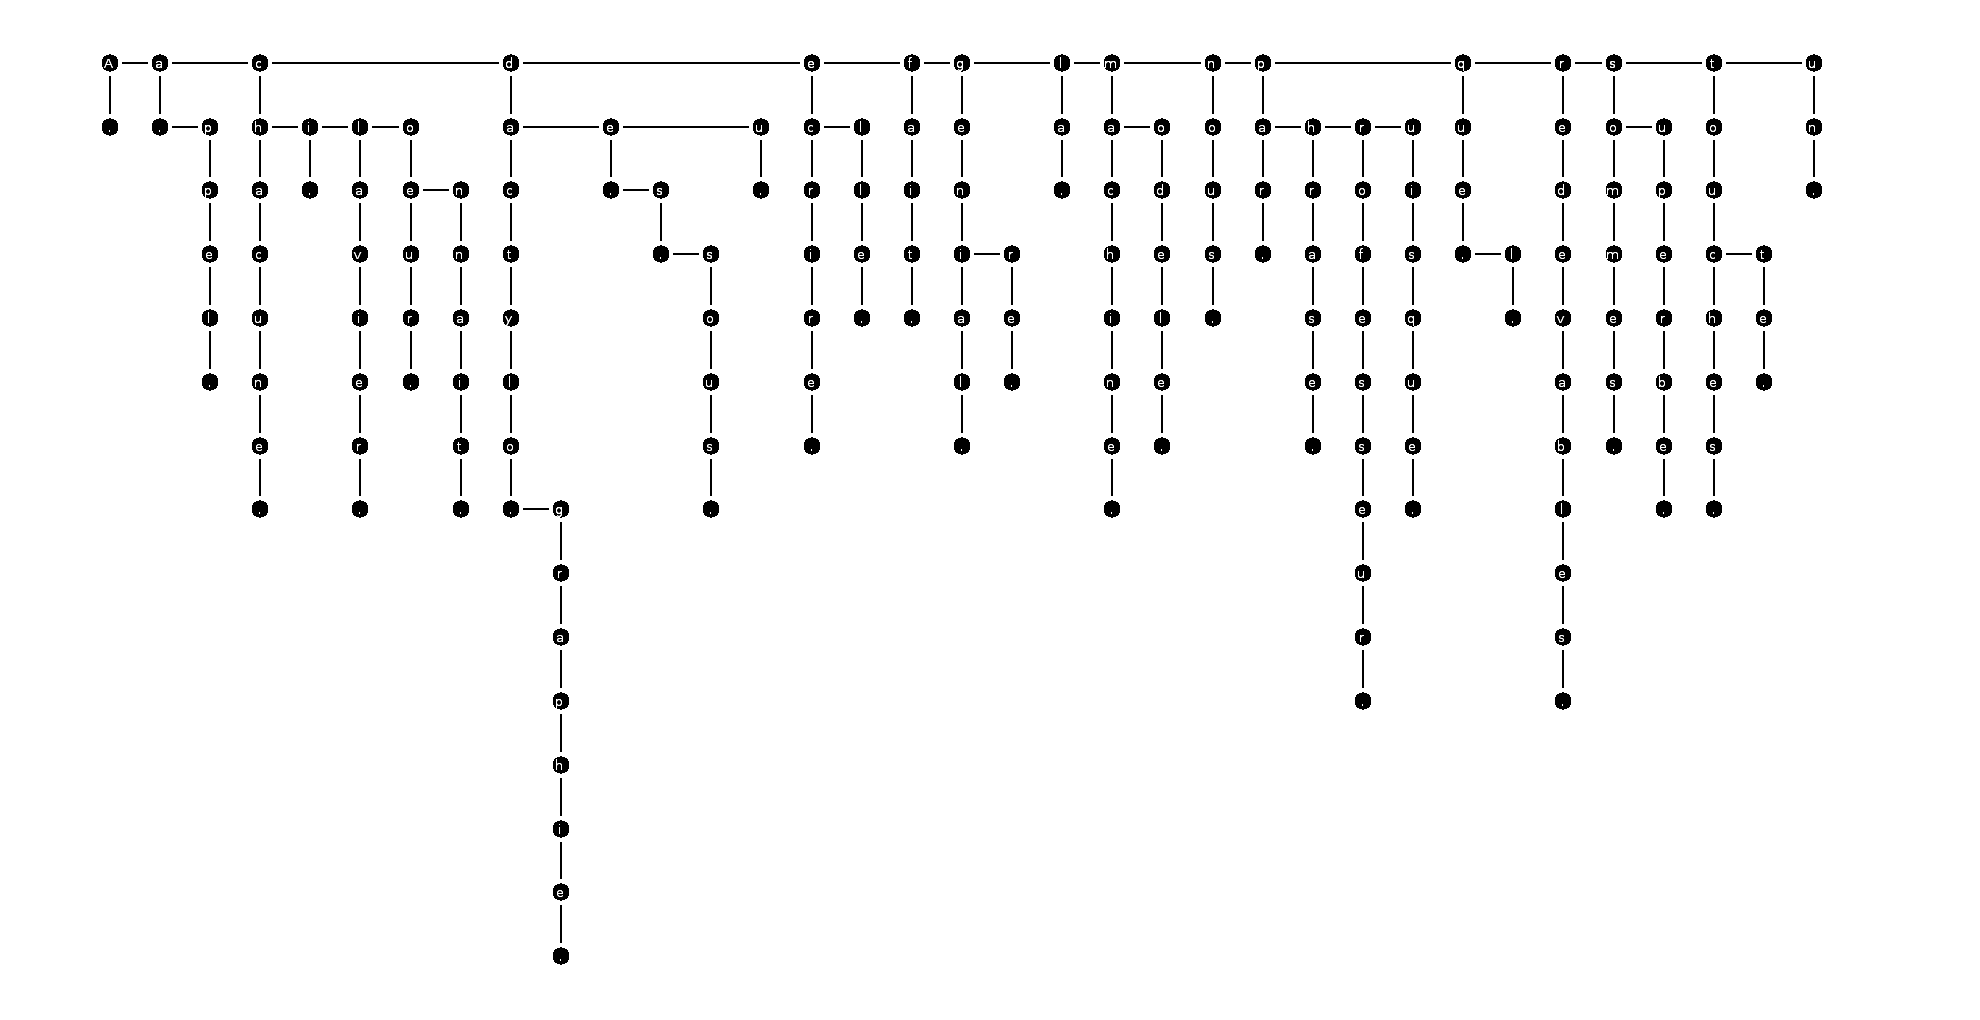
\includegraphics[width=1.1\textwidth]{briandais.png}
  \end{center}
\end{frame}

\subsection{Trie Hybride}
\begin{frame}
  \frametitle{Trie Hybride}
  \begin{center}
    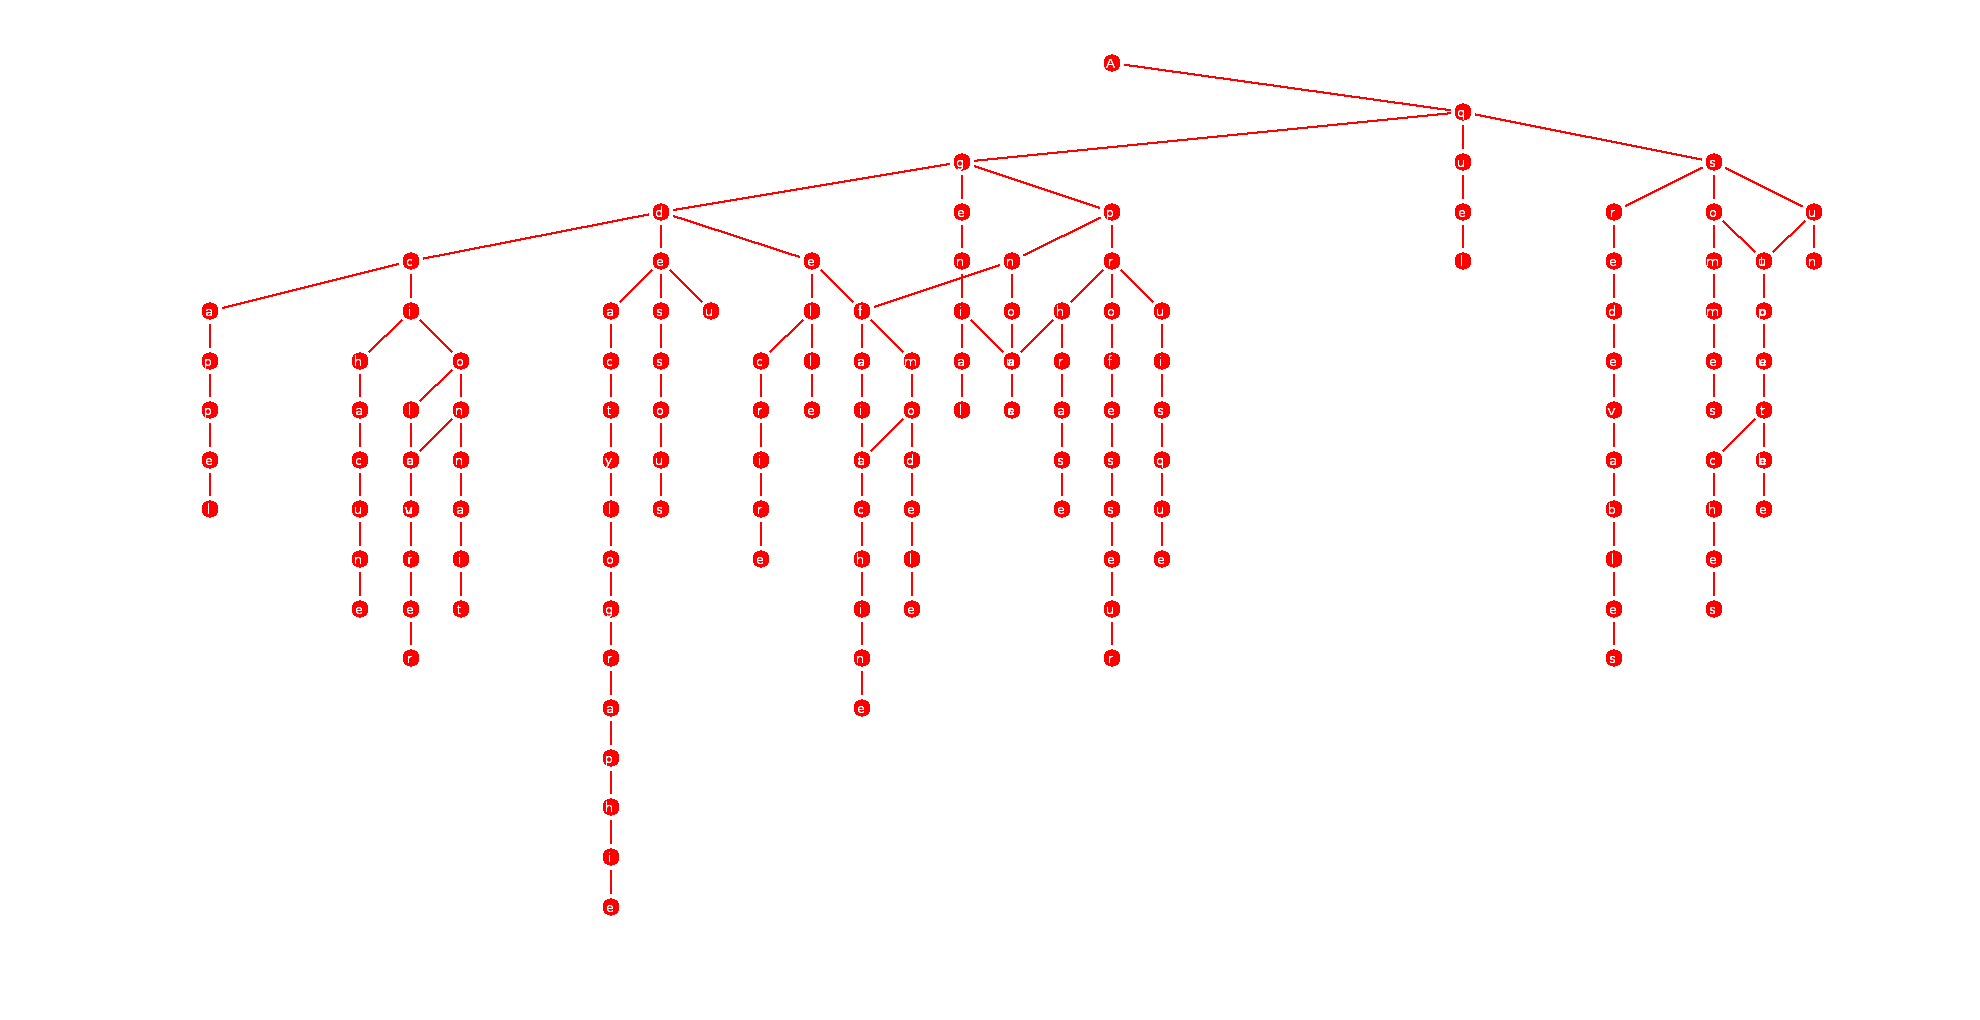
\includegraphics[width=1.1\textwidth]{hybrid.png}
  \end{center}
\end{frame}

\section{Temps de calcul}

\subsection{Temps pour l'ajout de mots}
\begin{frame}
  \frametitle{Ajout de mots}
  \begin{center}
    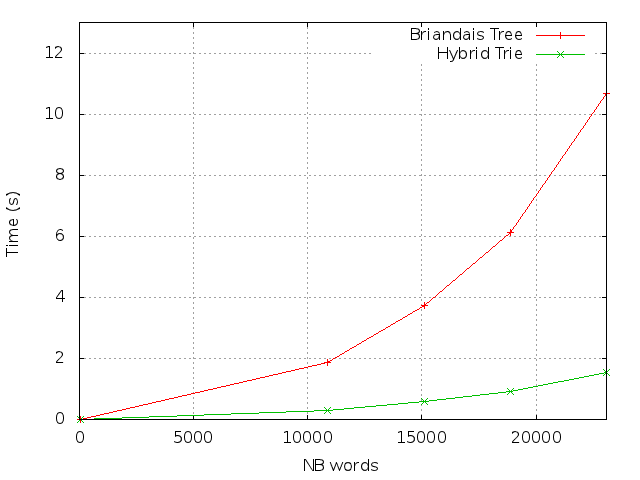
\includegraphics[width=0.8\textwidth]{timeAdd.png}
  \end{center}
\end{frame}

\subsection{Temps pour la suppression de mots}
\begin{frame}
  \frametitle{Suppression de mots}
  \begin{center}
    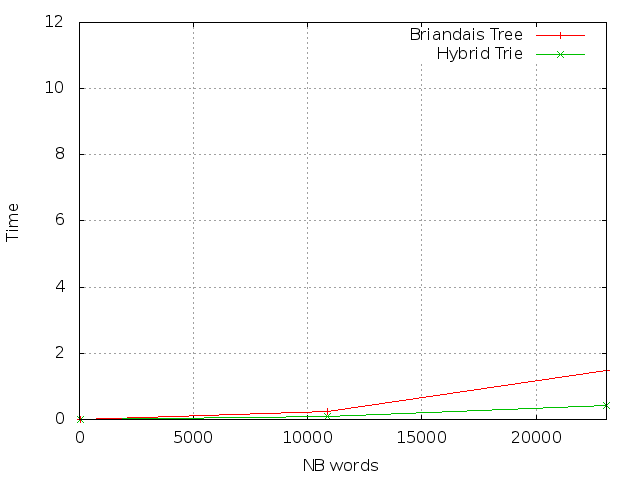
\includegraphics[width=0.8\textwidth]{timeDel.png}
  \end{center}
\end{frame}

\section{Parall\`elisme}
\subsection{Difference entre les deux m\'ethodes}
\begin{frame}
  \frametitle{Graphique avec et sans thread}
  \begin{center}
    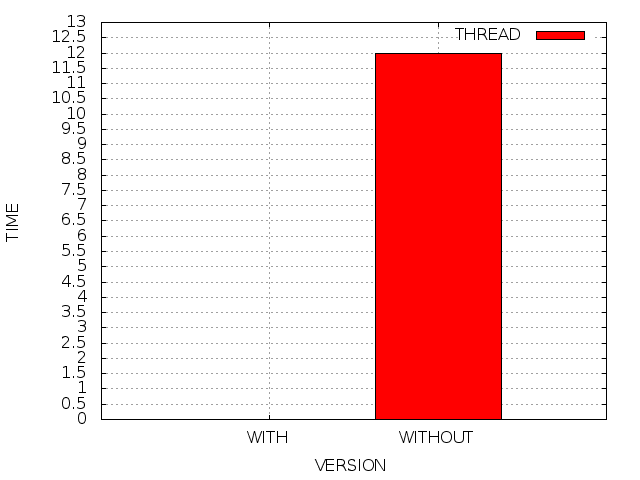
\includegraphics[width=0.8\textwidth]{thread.png}
  \end{center}
\end{frame}

\end{document}
